\par Aby możliwe było zrealizowanie przepływu informacji między grupami ludzi, konieczne jest przygotowanie systemu, który umożliwi komunikację elektroniczną oraz wymianę dokumentów. Komunikacja ta musi odbywać się poprzez system zapewniający bezpieczeństwo informacji, rozumiane jako kontrola dostępu do informacji i zabezpieczenie przed ich utratą. W tym celu należy utworzyć dwa podsystemy, z których jeden będzie odpowiedzialny za zbieranie zamówień i prezentowanie ofert klientom, drugi będzie odpowiadać za prawidłową obsługę procesów w firmie. Pierwszy z systemów nazywany będzie sklepem internetowym, drugi natomiast systemem zarządzania.
	
			\par Funkcjonowanie systemu zarządzania oraz sklepu internetowego wymaga następujących podsystemów pomocniczych: system wiadomości e-mail oraz system baz danych. System wiadomości e-mail odpowiada za przesyłanie korespondencji elektronicznej, natomiast system baz danych za przechowywanie danych pochodzących z poprzednich systemów. 
			%Należy jeszcze sformułować dla tych systemów kroki niezbędne celem zapewnienia bezpieczeństwa i spójności danych.
		
			\par Wymagane elementy można przedstawić za pomocą następującego schematu, w którym strzałki oznaczają przepływ informacji.
		
			\begin{figure}[H]
				\centering
				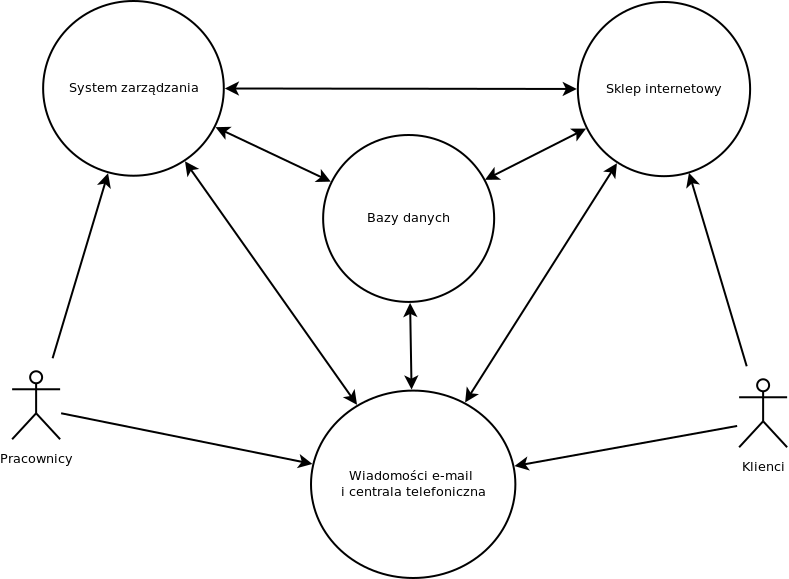
\includegraphics[scale=0.45]{basic_component}
				\caption{Schemat komunikacji poprzez sieć firmową}
				\label{basic_comp}
			\end{figure}
		
			\par Rysunek przedstawia podstawowy diagram przepływu informacji pomiędzy komponentami systemu. Głównym jego elementem jest tu system zarządzania oraz sklep internetowy. System baz danych oraz wiadomości elektronicznych są elementami wymaganymi dla działania dwóch głównych komponentów. Jak pokazuje schemat, dane z systemu zarządzania i sklepu internetowego zapisywane są w bazie danych. Systemy te generują wiadomości e-mail, obsługiwane przez system wiadomości e-mail, który przychodzącą i wychodzącą korespondencje zapisuje w bazie danych. Klienci komunikują się z przedsiębiorstwem poprzez sklep internetowy, wiadomości e-mail oraz rozmowy telefoniczne, natomiast pracownicy przez system zarządzania, wiadomości e-mail i rozmowy telefoniczne.
 
